\documentclass[11pt]{scrartcl}
\usepackage[utf8]{inputenc}
\usepackage{evank}


%% insert title here
\newcommand{\titlee}{AC Circuits}
\parindent 0 pt

\newcommand{\officialsol}[1]{See the official solutions \href{#1}{here}.}

\title{\titlee}
\author{Cambridge Physics Academy}
\date{2023-2024}


\begin{document}

\thispagestyle{empty}
\begin{center}
    
    
    \Huge \textbf{\textsf{\titlee}}

    \large \theauthor
\end{center}

\setcounter{section}{-1}
\section{Readings}
\begin{itemize}
    \item Ch 37 of HRK
    \item Ch 8 of Purcell
\end{itemize}
Feel free to do problems from the readings as extra practice.


\section{Lecture review}

\begin{theorem}[Undriven RLC oscillators]\label{undriv}
    For an undriven RLC oscillator, the differential equation corresponding to Kirchoff's law is $$\ddot q+\frac{R}{L}\dot q+\frac{1}{LC}q=0$$ Let $\gamma=R/2L$ and $\omega_0^2=1/LC$. The general solution to this differential equation is  $$q(t)=q_0e^{-\gamma t}\cos(t\sqrt{\omega_0^2-\gamma^2}+\varphi)$$ See Problem \ref{deriv} below for a derivation.
\end{theorem}

\begin{theorem}[Driven RLC oscillators]\label{driven}
    A driven oscillator contains a time-dependent sinusoidal voltage source $$\mathcal E(t)=\mathcal E_0\cos\omega t$$ We can substitute this voltage with a complex voltage $\mathcal E_0e^{i\omega t}$, and solve the system in terms of these complex values. The oscillation frequency of the current will match the oscillation frequency of the voltage, so we take $I(t)=\tilde Ie^{i\omega t}$ where $\tilde I$ is the fixed vector $\tilde I=I_0e^{i\varphi}$ in the complex plane. Plugging this into Kirchoff's law yields $$Li\omega\tilde Ie^{i\omega t}+R\tilde Ie^{i\omega t}+\frac{1}{i\omega C}\tilde Ie^{i\omega t}=\mathcal E_0e^{i\omega t}$$Which we can use to find $$I_0=\frac{\mathcal E_0}{\sqrt{R^2+(\omega L-1/\omega C)^2}}\qquad \tan\varphi=\frac{1}{R\omega C}-\frac{\omega L}{R}$$
\end{theorem}

\begin{theorem}[Impedance]
    We can substitute a capacitor $C$ and an inductor $L$ in a circuit as effective resistors with impedances $$Z_L=i\omega L\qquad Z_C=\frac{1}{i\omega C}$$
\end{theorem}

\begin{idea}[Phasors]
    A helpful way of analyzing circuits is using impedances and phasors on the complex plane. The general idea is as such: \begin{enumerate}
        \item Draw the phasor for the current $I$ at an angle of 0 degrees for ease of analysis.
        \item Draw phasors representing the voltages across each of the circuit components by using $V=IZ$. 
        \item The sum of these phasors will yield the net voltage phasor across the components (if they are connected with series).
        \item From this we can extrapolate the phase angle $\varphi$ and the amplitude of $I$ from the voltage amplitude. 
    \end{enumerate}
\end{idea}

\begin{defn}[RMS]
Since the explicit average of current and voltage in an alternating circuit is 0, we use the root-mean square value to represent an average. The RMS is defined as $$V_{\text{rms}}=\sqrt{\overline{V^2}}$$
\end{defn}

\begin{theorem}[Power]
    The average power dissipation in a circuit is given by the RMS voltage on the voltage source and the RMS current passing through it: $$P=\mathcal E_{\text{rms}}I_{\text{rms}}\cos\varphi$$Note $\varphi$ is the phase difference between $\mathcal E(t)$ and $I(t)$. A derivation is found in Problem \ref{powah}.
\end{theorem}
\section{Problem Set}

\subsection{Exercises}

\begin{prob}\label{deriv}
    It's helpful to run through the precise derivation of an RLC oscillator at least once. We'll do that in this problem. Assume we have a resistor $R$, inductor $L$, and capactor $C$ connected in series. 
    \begin{anum}
        \item Using Kirchoff's law, write a differential equation in terms of $q$, the charge on the capacitor, and its derivatives. 
        \item Now, guess the solution $q=q_0e^{i\omega t}$ and plug this into your equation. You should get a quadratic in $\omega$. Solve this quadratic to find two solutions for $\omega$.
        \item The property of linearity (that we're dealing with a linear differential equation) guarantees that the most general solution to $q$ is some linear combination of the two solutions you found in part (b). Write the most general solution in terms of two linear coefficients $A$ and $B$.
    \end{anum}
\end{prob}

\begin{sol}
    \begin{anum}
        \item The net voltage in the loop is 0, so by the loop rule $$\boxed{\ddot q+\frac{R}{L}\dot q+\frac{1}{LC}q=0}\Rightarrow \ddot q+2\gamma \dot q+\omega_0^2 q=0$$where we used the substitutions $\gamma=R/2L$ and $\omega_0^2=1/LC$. 
        \item Taking the derivatives, $\dot q=i\omega q_0e^{i\omega t}$ and $\ddot q=-\omega^2q_0e^{i\omega t}$. Plugging these in, all the $q_0e^{i\omega t}$ cancel out, so $$-\omega^2+2\gamma i\omega +\omega_0^2=0$$By the quadratic formula, $$\omega=\boxed{i\gamma \pm \sqrt{\omega_0^2-\gamma^2}}$$
        \item Plugging $\omega$ in, our two possible solutions are $$q_1=q_0e^{(-\gamma+i\sqrt{\omega_0^2-\gamma^2})t}\qquad q_2=q_0e^{(-\gamma-i\sqrt{\omega_0^2-\gamma^2})t}$$So the most general solution is $$q=\boxed{q_0e^{-\gamma t}(Ae^{i\sqrt{\omega_0^2-\gamma^2}t}+Be^{-i\sqrt{\omega_0^2-\gamma^2}t})}$$With Euler's identity and a few trigonometric identities we can create the result in Theorem \ref{undriv}.
    \end{anum}
\end{sol}

\begin{prob}
    An RLC oscillator is critically damped when $R=2\sqrt{L/C}$. In turns out that in this case the general solution to $q$ takes the form $$q(t)=(A+Bt)e^{-\beta t}$$for constants $A$, $B$, $\beta$. \begin{anum}
        \item Find $\beta$.
        \item Initially at $t=0$ let current $I_0$ flow through the circuit and let there be charge $q_0$ on the capacitor. Using this information, find $q(t)$ in terms of $R$, $L$, $C$, and the initial conditions. 
    \end{anum} 
\end{prob}

\begin{sol}
    \begin{anum}
        \item Using $R=2\sqrt{L/C}$ our differential equation becomes $$\ddot q+\frac{2}{\sqrt{LC}}\dot q+\frac{1}{LC}q=0$$Taking the derivatives of $q$, we get $\dot q=-e^{-\beta t}(A\beta-B+B\beta t)$ and $\ddot q=\beta e^{-\beta t}(A\beta -2B+B\beta t)$. Plugging these in, $A$ cannot depend on $B$ so the coefficients in front of the $A$'s must sum to 0: $$\beta^2-\frac{2}{\sqrt{LC}}\beta+\frac{1}{LC}=0\Rightarrow \beta=\boxed{\frac{1}{\sqrt{LC}}}$$
        \item Substituting $t=0$ for $q$, we have $A=q_0$. Using our derivative $\dot q$ from earlier, $B-A\beta=I_0\Rightarrow B=I_0+q_0/\sqrt{LC}$. Plugging these in yields $$q(t)=\boxed{\left[q_0+t\left(I_0+\frac{q_0}{\sqrt{LC}}\right)\right]e^{-t/\sqrt{LC}}}$$
    \end{anum}
\end{sol}

\begin{prob}
    For a resistor $R$, inductor $L$, and capacitor $C$ connected in parallel, what is their effective impedance? 
\end{prob}

\begin{sol}
    Using the formula for resistances added in parallel, $$Z=\boxed{\frac{1}{1/R+1/i\omega L+i\omega C}}$$
\end{sol}

\begin{prob}[Purcell]
    Is it possible to find a nontrivial frequency at which the impedance at the terminals of the circuit in the figure below will be purely real?
    \begin{center}
        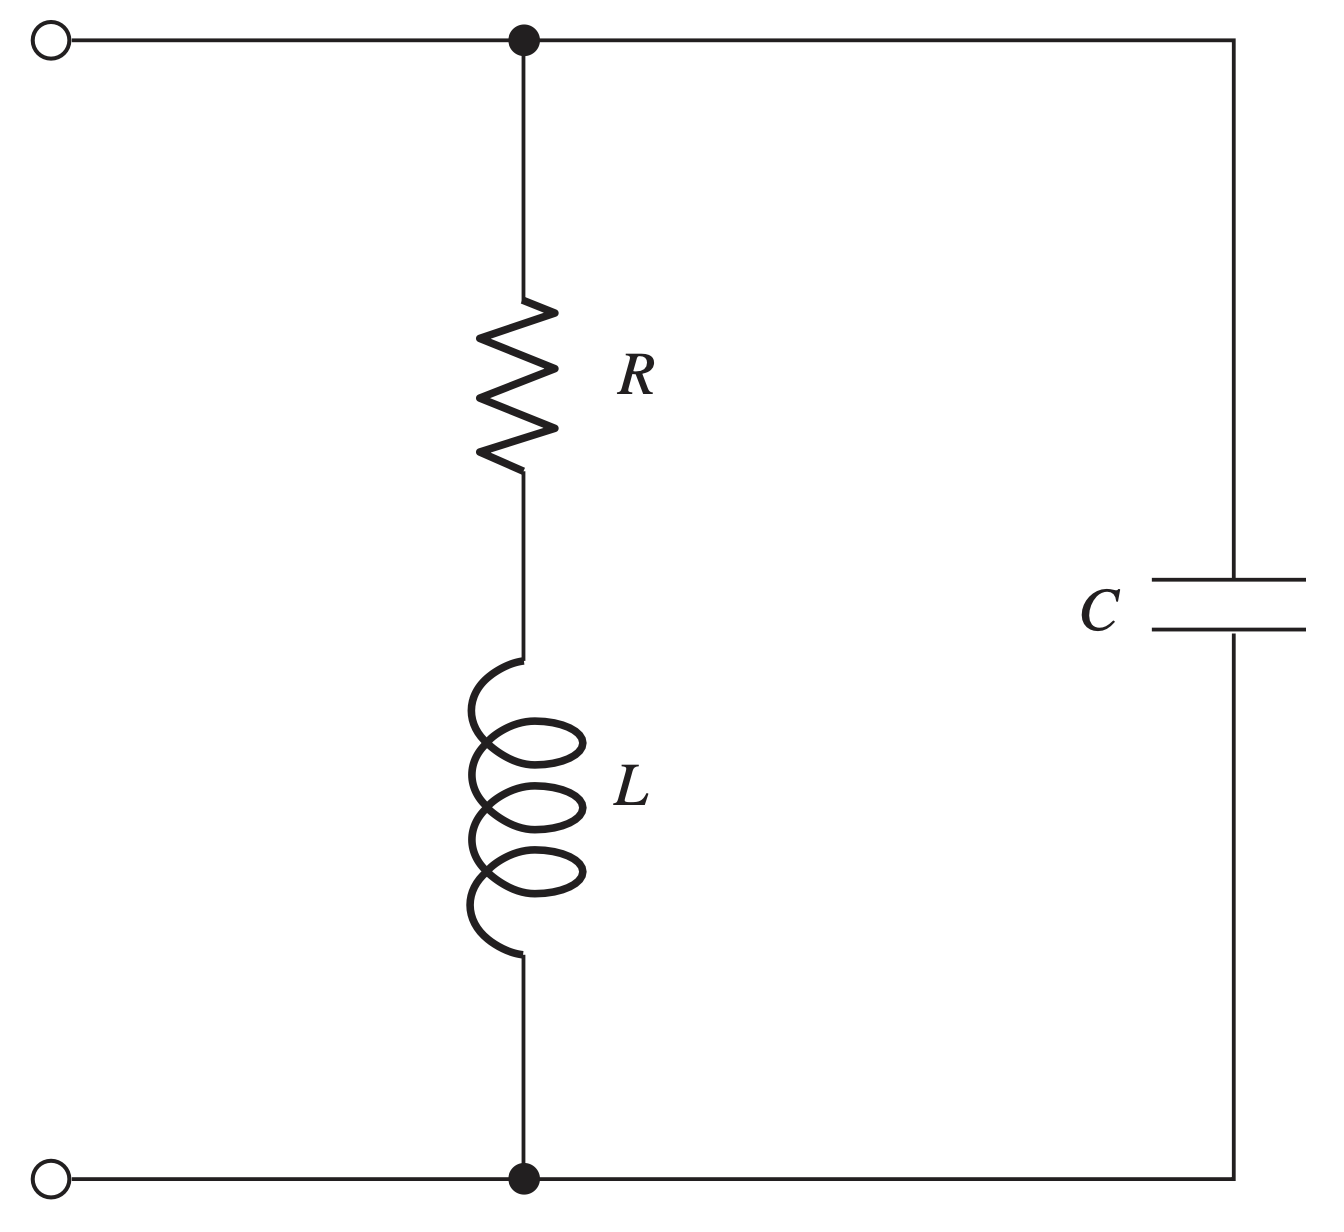
\includegraphics[scale=0.25]{purcell1}
    \end{center}
\end{prob}

\begin{sol}
    The impedance is $$Z=\frac{1}{1/(R+i\omega L)+i\omega C}$$The impedance is real if its reciprocal is real: $$\frac1Z=\frac{1}{R+i\omega L}+i\omega C=\frac{R-i\omega L}{R^2+\omega^2L^2}+i\omega C$$Setting the imaginary part equal to 0 yields $$\frac{\omega L}{R^2+\omega^2L^2}=\omega C\Rightarrow \omega=\sqrt{\frac{1}{LC}-\frac{R^2}{L^2}}$$so yes, \fbox{there is such a frequency} so long as $R^2<L/C$. 
\end{sol}

\begin{prob}[Purcell]\label{lowpass}
In the figure below an alternating voltage $V_0\cos\omega t$ is applied to the terminals at $A$. The terminals at $B$ are connected to an audio amplifier of very high input impedance. (That is, current flow into the amplifier is negligible.) Calculate the ratio $|\tilde V_1|^2/V_0^2$. Here $|\tilde V_1|$ is the absolute value of the complex voltage amplitude at terminals $B$. Choose values for $R$ and $C$ to make $|\tilde V_1|^2/V_0^2=0.1$ for a 5000 Hz signal. This circuit is the most primitive of ``low-pass" filters, providing attenuation that increases with increasing frequency. Show that, for sufficiently high frequencies, the signal power is reduced by a factor $1/4$ for every doubling of the frequency.
\begin{center}
    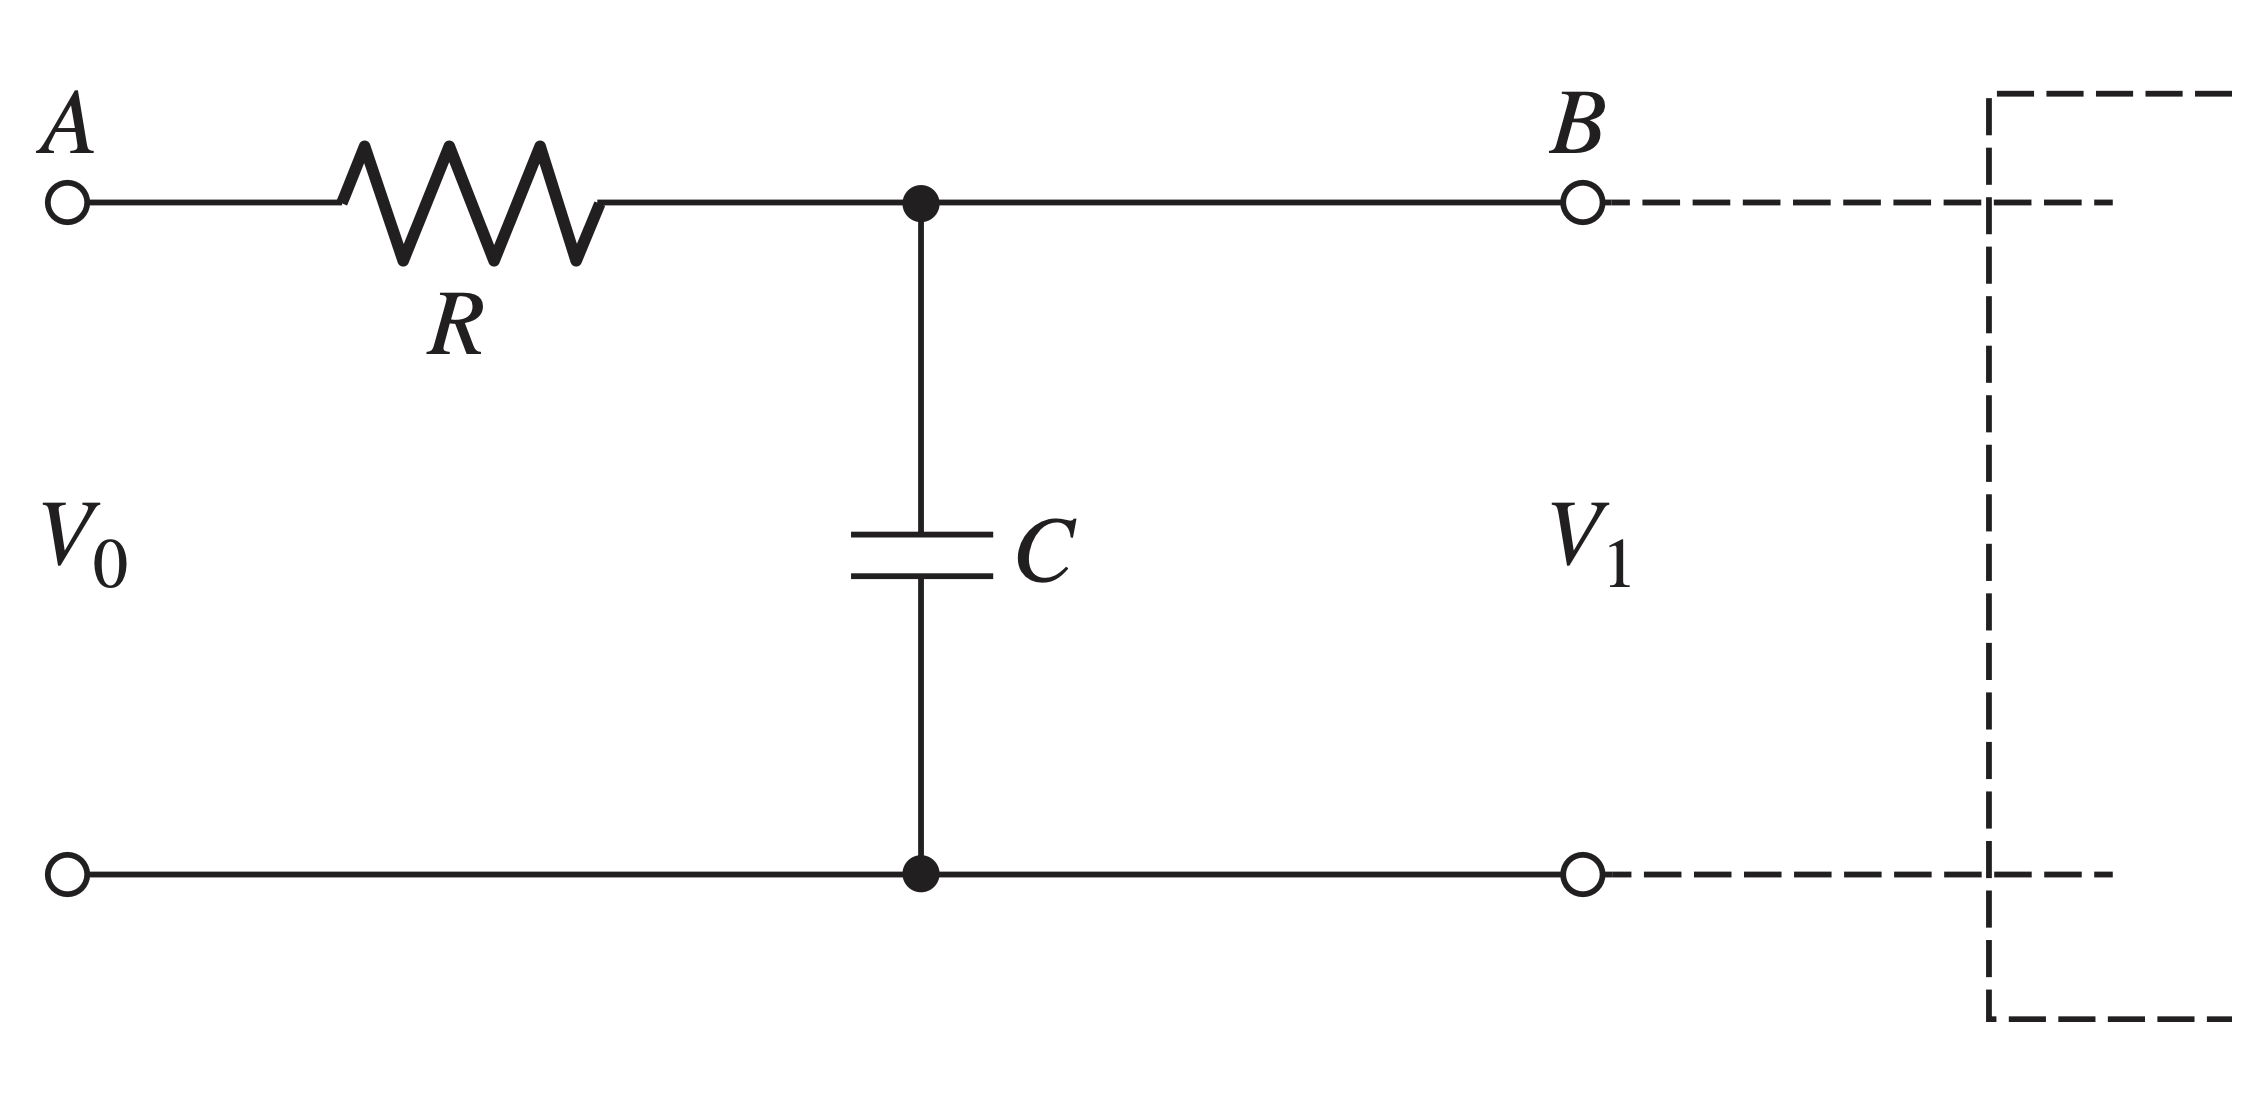
\includegraphics[scale=0.2]{purcell2}
\end{center}
\end{prob}

\begin{sol}
    Let $I_0$ be the amplitude of the current through the resistor, which is also essentially the current through the capacitor. Then the complex $\tilde V = \tilde IZ$ statement for the voltage between the terminals at $A$ is $V_0 = \tilde I(R+1/i\omega C)$. And the statement for the terminals at $B$ is $\tilde V_1= \tilde I(1/i\omega C)$. Therefore, $$\frac{\tilde V_1}{V_0}=\frac{1}{1+i\omega RC}\Rightarrow \left|\frac{\tilde V_1}{V_0}\right|^2=\boxed{\frac{1}{1+\omega^2 R^2C^2}}$$This equals 0.1 when $\omega^2 R^2C^2 = 9$, so at $\omega= 5000\, \unit{Hz}$ this gives $$RC=\frac{3}{\omega}=\frac{3}{2\pi \cdot 5000\, \unit{s^{-1}}}\approx \boxed{1\cdot 10^{-4}\, \unit s}$$ The power is proportional to $V^2$. If $\omega$ is large, we can ignore the 1 in the denominator of our result for the ratio $|\tilde V_1|^2/V_0^2$. We then have $|\tilde V_1/V_0|^2\propto 1/\omega^2$. Doubling $\omega$ decreases this by a factor of 4.
\end{sol}

\begin{prob}
    Taking inspiration from Problem \ref{lowpass}, sketch a simple circuit that could act as a high-pass filter, where the output is amplified with higher frequencies. Calculate the ratio $|\tilde V_1|^2/V_0^2$ in terms of the parameters in your new circuit. 
\end{prob}

\begin{sol}
    We take the same circuit in Problem \ref{lowpass}, but replace the capacitor with an inductor $L$. Then $V_0=\tilde I(R+i\omega L)$ and $\tilde V_1=\tilde Ii\omega L$. Therefore, $$\frac{\tilde V_1}{V_0}=\frac{1}{1+(R/i\omega L)}\Rightarrow \left|\frac{\tilde V_1}{V_0}\right|^2=\boxed{\frac{1}{1+(R/\omega L)^2}}$$
\end{sol}

\begin{prob}
    In the circuit below, let $I_L$ be the current passing through the branch with the inductor, and let $I_C$ be the current passing through the branch with the capacitor. The input voltage is $\mathcal E(t)=\mathcal E_0\cos\omega t$.
    \begin{center}
        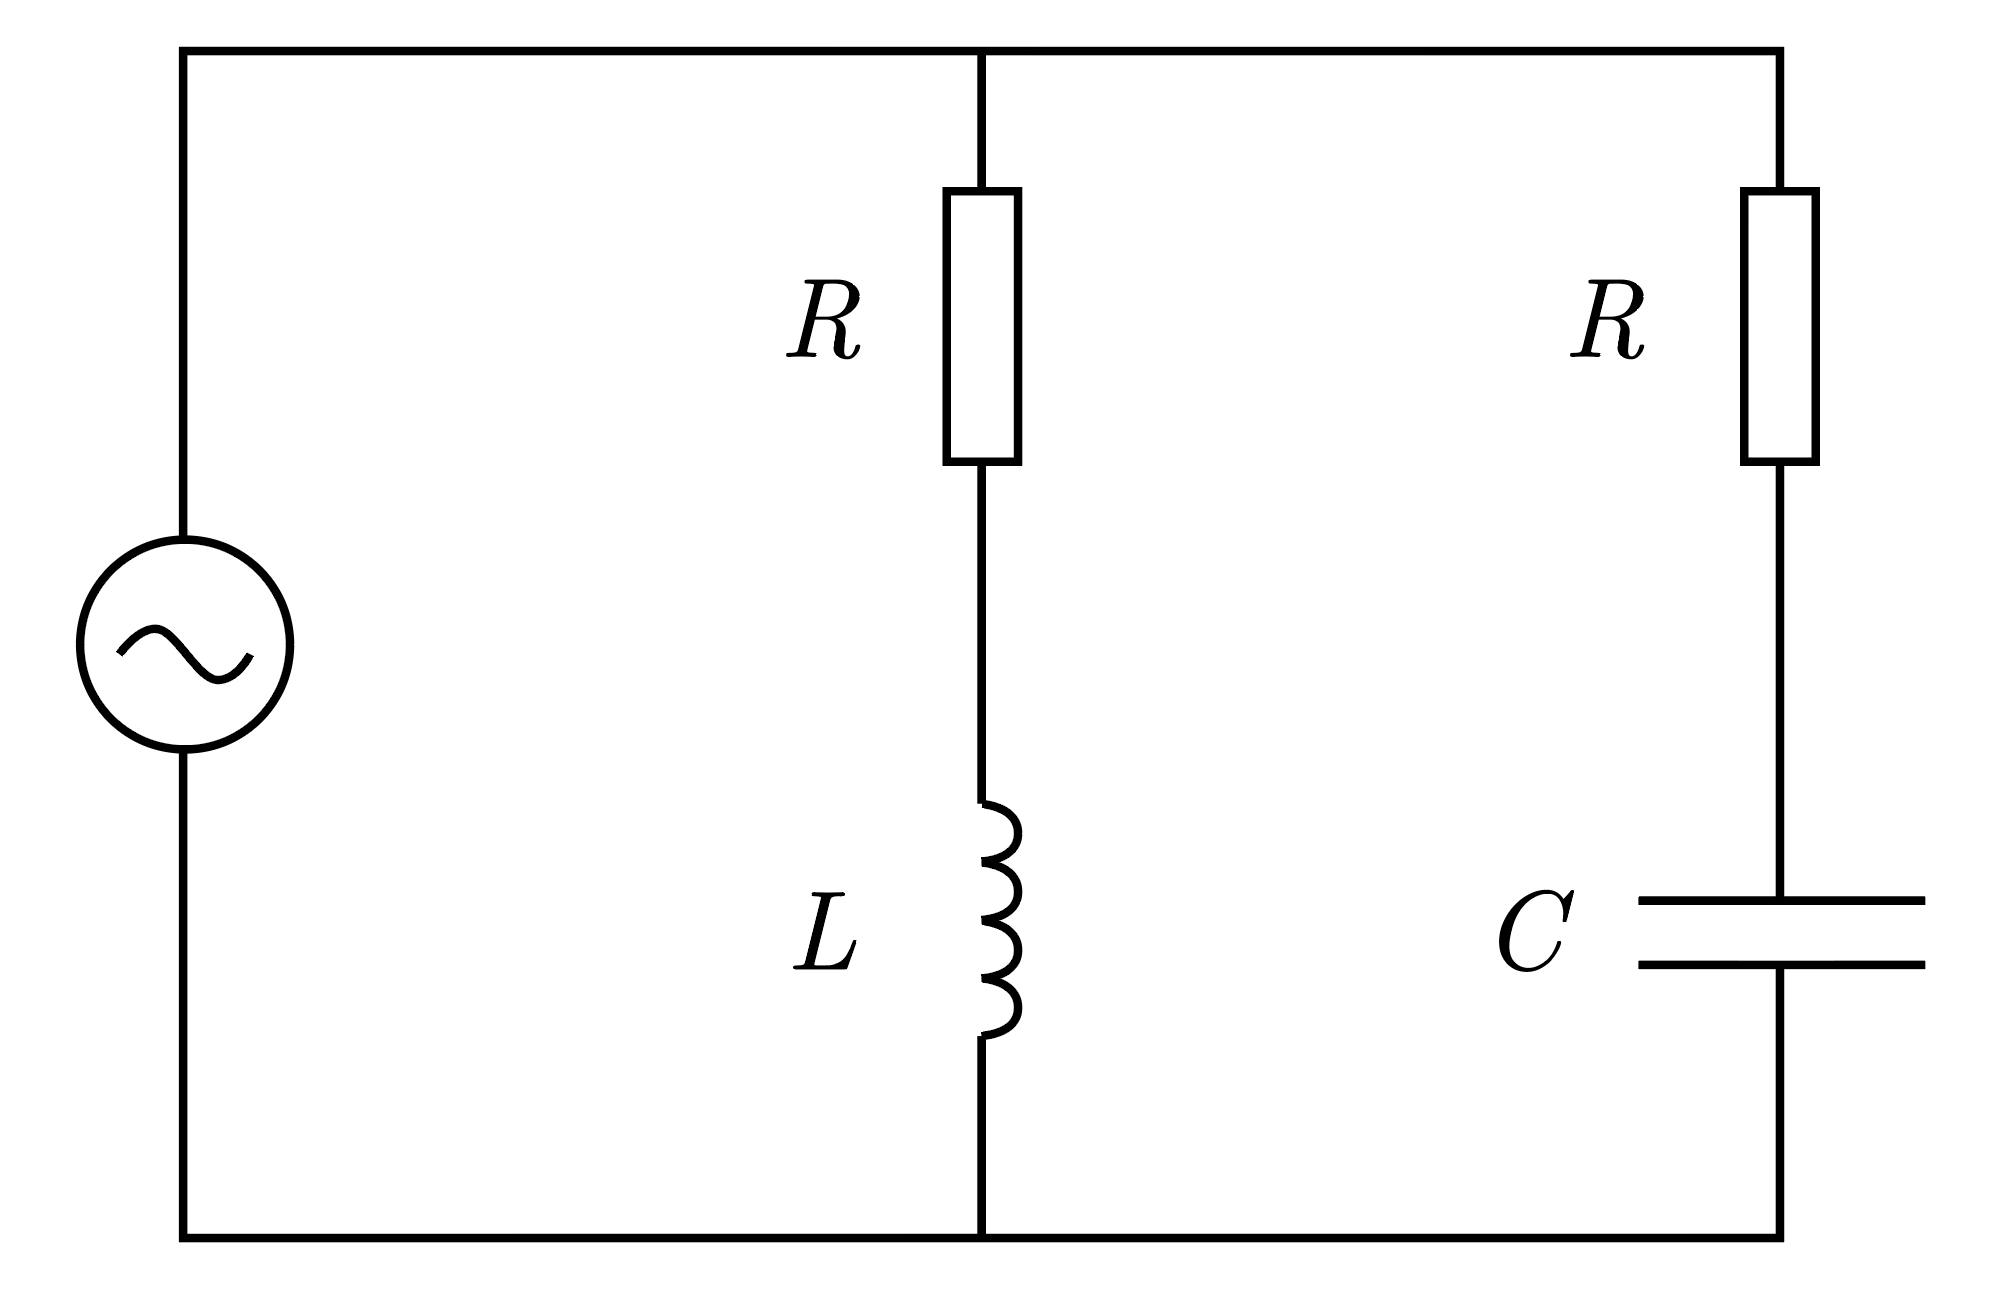
\includegraphics[scale=0.2]{rlc}
    \end{center}
    \begin{anum}
        \item At very high frequencies $\omega \gg 1$, find $I_L$ and $I_C$ as a function of time. 
        \item At very low frequencies $\omega \ll 1$, find $I_L$ and $I_C$ as a function of time.
        \item Now assume general values of $\omega$. What is the phase difference between $I_L$ and $I_C$?
        \item Find $I_L$ and $I_C$ as a function of time for general $\omega$. Check that in the limits of parts (a) and (b), your results reduce to the correct values. 
        \item At what $\omega$ does the whole system behave like a resistor? 
    \end{anum}
\end{prob}

\begin{sol}
    \begin{anum}
        \item For very high frequencies, the impedance of the inductor is infinite so $\boxed{I_L=0}$. Then, we neglect the impedance of the capacitor so $\boxed{I_C=(\mathcal E_0/R)\cos\omega t}$.
        \item We simply swap our answers from (a): $\boxed{I_L=(\mathcal E_0/R)\cos\omega t}$ and $\boxed{I_C=0}$.
        \item Note that the voltage across each branch must be the same. Given the following phasor diagram: \begin{center}
            
\includegraphics[scale=0.2]{sol1}
        \end{center}
        The currents point in the directions of the $R$ vectors, so the phase difference is the angle between the two vectors going off on the left. Thus by some trig the phase difference is $$\varphi=\boxed{\tan^{-1}\left(\frac{1}{\omega RC}\right)+\tan^{-1}\left(\frac{\omega L}{R}\right)}$$
        \item From the right triangles, the amplitude of $I_C$ is $\mathcal E_0/\sqrt{R^2+(1/\omega C)^2}$ and the amplitude of $I_L$ is $\mathcal E_0/\sqrt{R^2+(\omega L)^2}$. The phase differences are the individual components of our answer to part (c). Thus \begin{gather*}\boxed{I_C=\frac{\mathcal E_0}{\sqrt{R^2+(1/\omega C)^2}}\cos\left[\omega t+\tan^{-1}\left(\frac{1}{\omega RC}\right)\right]}\\
        \boxed{I_L=\frac{\mathcal E_0}{\sqrt{R^2+(\omega L)^2}}\cos\left[\omega t-\tan^{-1}\left(\frac{\omega L}{R}\right)\right]}\end{gather*}As expected the amplitudes and phase shifts reduce to the limits we expect from parts (a) and (b). 
        \item We want the total impedance to have no imaginary part. The impedance is real if the reciprocal is real, so $$\frac1Z=\frac{1}{R+i\omega L}+\frac{1}{R+(1/i\omega C)}=\frac{R-i\omega L}{R^2+\omega^2L^2}+\frac{R+i/\omega C}{R^2+(1/\omega C)^2}$$ Setting the imaginary part equal to 0 yields $$\frac{1}{\omega C(R^2+1/\omega^2C^2)}-\frac{\omega L}{R^2+\omega^2L^2}\Rightarrow\omega=\boxed{\sqrt{\frac{L-CR^2}{LC(L+CR^2)}}}$$
    \end{anum}
\end{sol}

\begin{prob}[NBPhO]
    Examine the circuit below.
    \begin{center}
        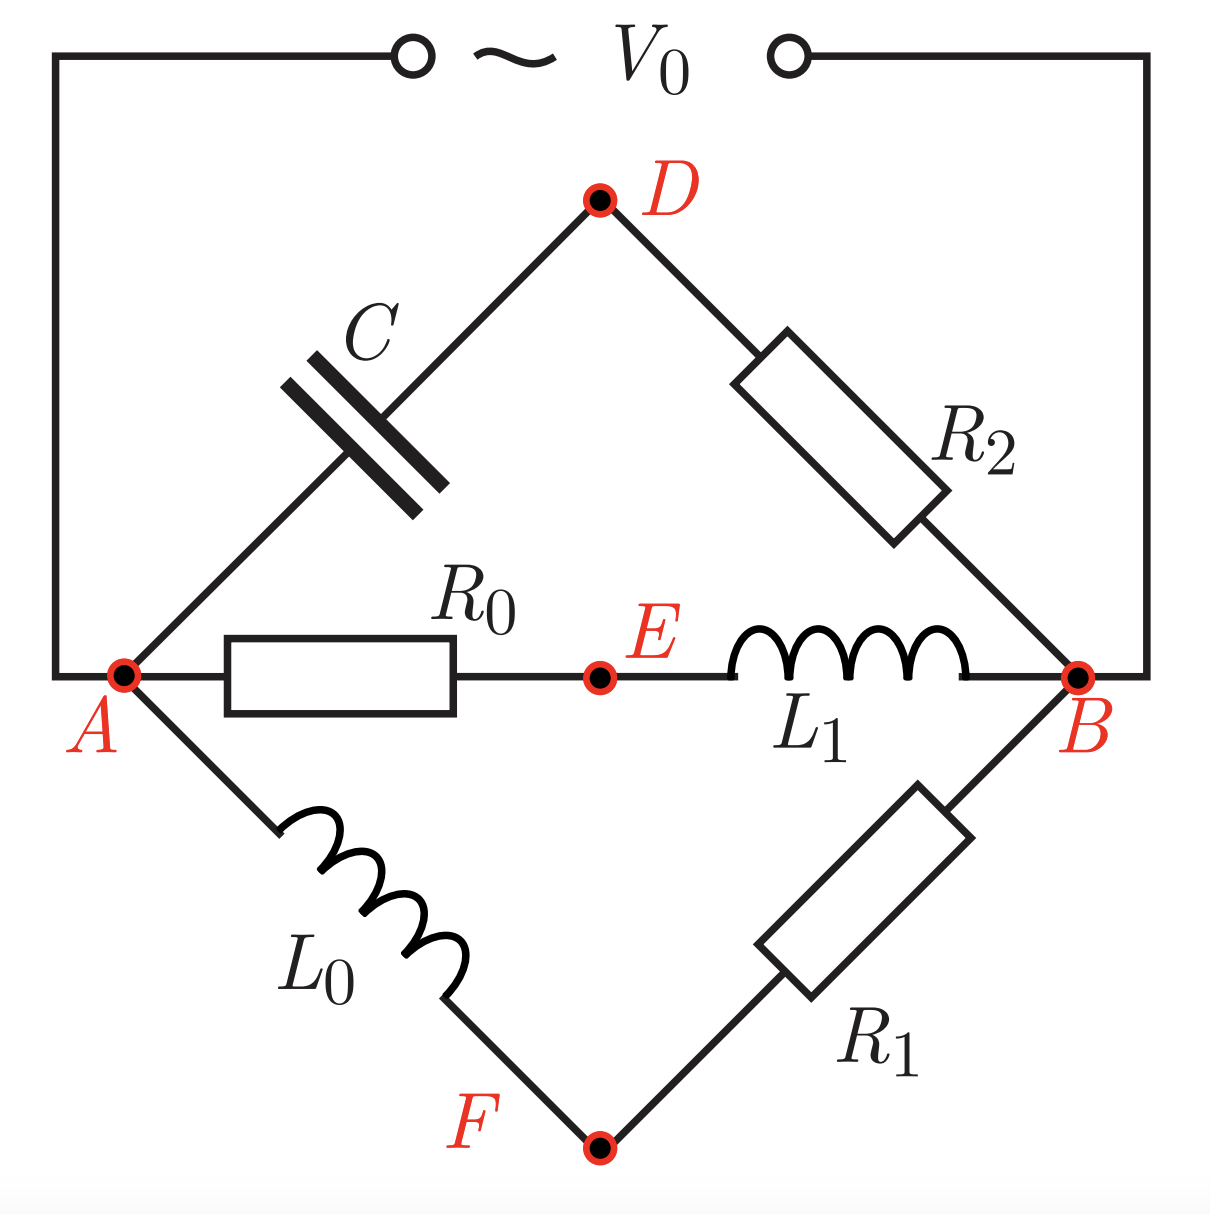
\includegraphics[scale=0.25]{kzldq}
    \end{center}
    \begin{anum}
    \item Draw a phasor diagram for this circuit showing the voltage vectors between the following nodes: $V_{AD}$, $V_{DB}$, $V_{AB}$, $V_{AE}$, $V_{EB}$, $V_{AF}$, and $V_{FB}$.
    \item The voltages between the nodes $D$, $E$, and $F$ are know to have the following values: $V_{DE} = 7\, \unit{V}$, $V_{DF} = 15\, \unit V$, and $V_{EF} = 20\, \unit V$; what is the value of the input voltage $V_0$? Hint: The radius of the circumcircle of a triangle with side lengths $a$, $b$, $c$ and area $A$ is $R=abc/4A.$
    \end{anum}
\end{prob}

\begin{sol}
    See solutions \href{https://www.ioc.ee/~kalda/ipho/es/NBPhO18_sol.pdf}{here}.
\end{sol}

\begin{prob}[USAPhO]
    The input voltage is the voltage difference between points I and II. Let $R_1C_1=R_2C_2$. What is the voltage difference between the points $a$ and $b$ in the circuit below as a function of time?
    \begin{center}
        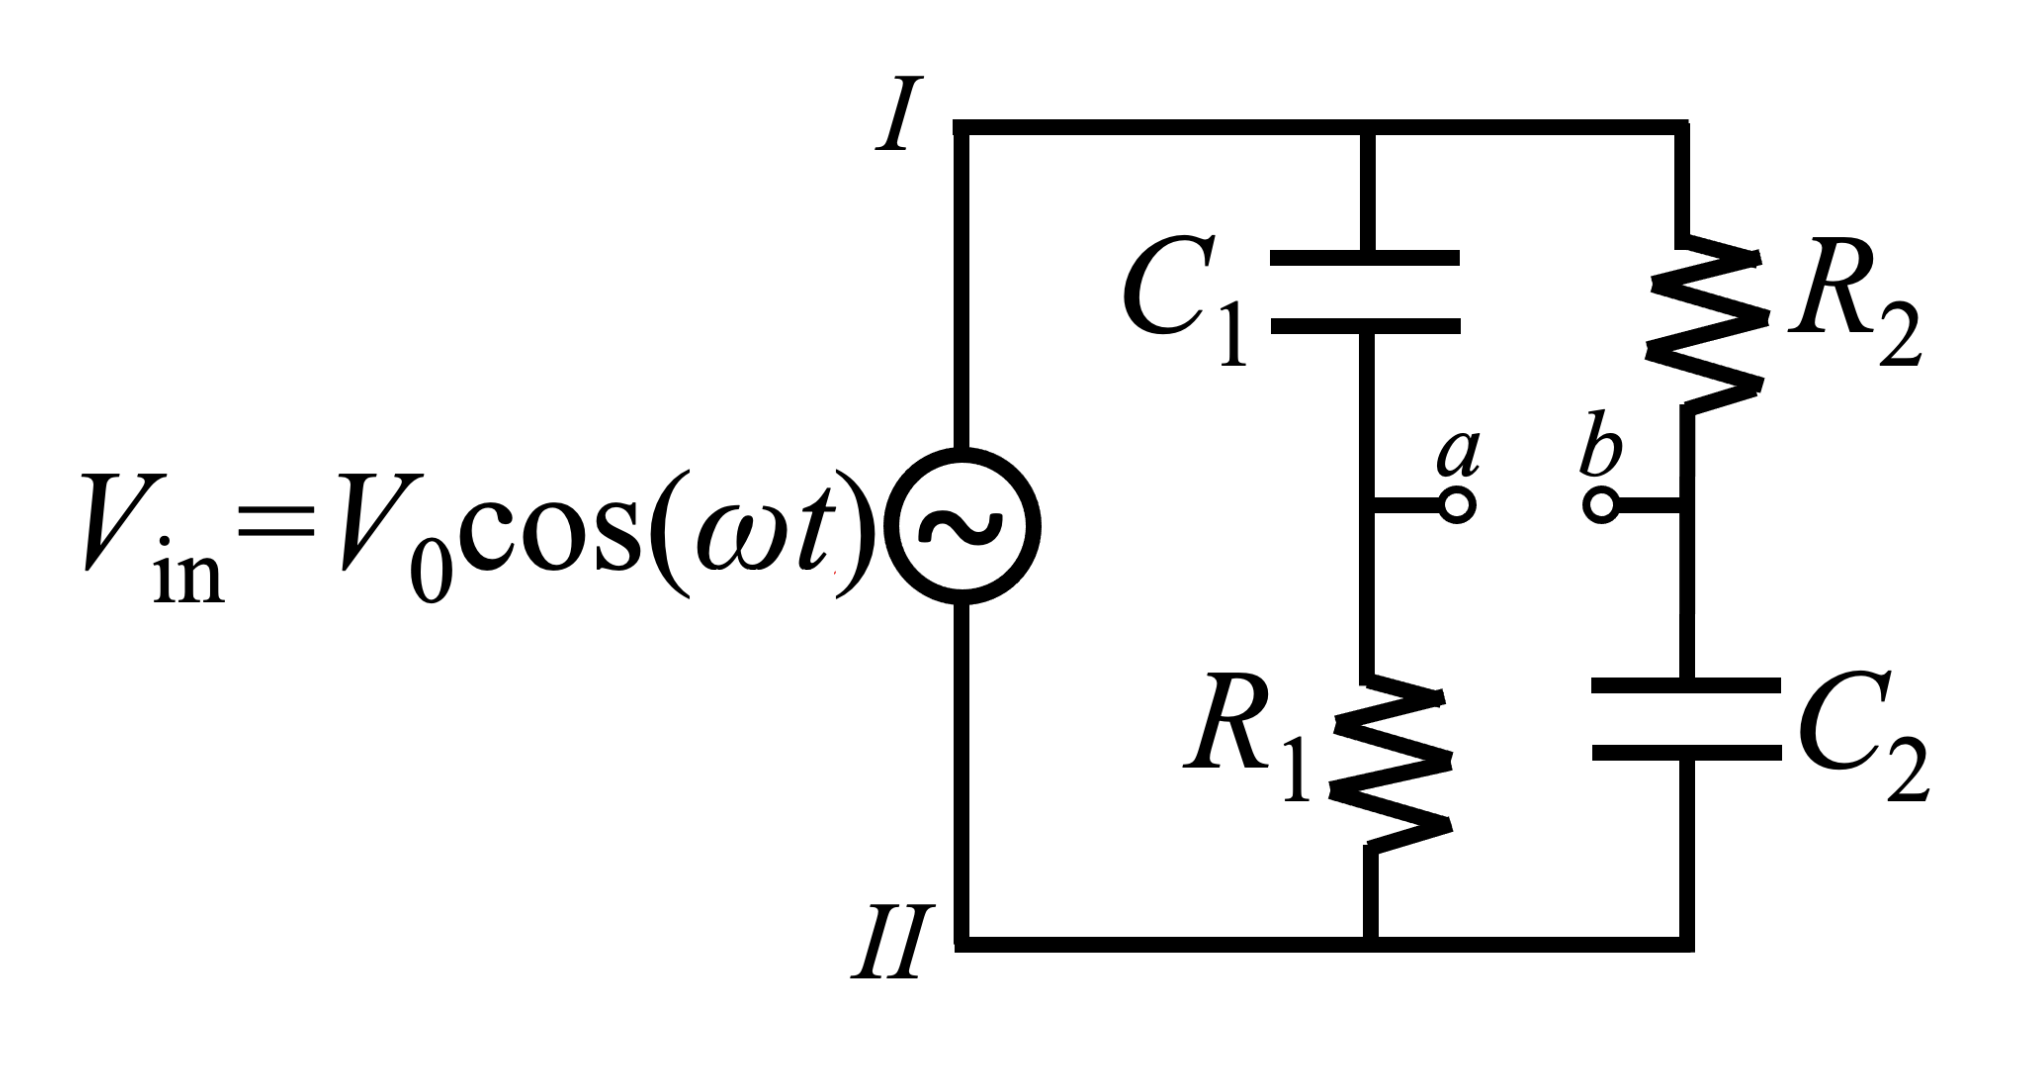
\includegraphics[scale=0.2]{uspe3}
    \end{center}
\end{prob}

\begin{sol}
    See solutions \href{https://aapt.org/physicsteam/upload/2022_Theory_TST_Solutions.pdf}{here} (Problem 1, Part 4).
\end{sol}

\begin{prob}[NBPhO]
An alternating voltage with amplitude $V_0$ and circular frequency $\omega_0$ is applied to the circuit shown below.
\begin{center}
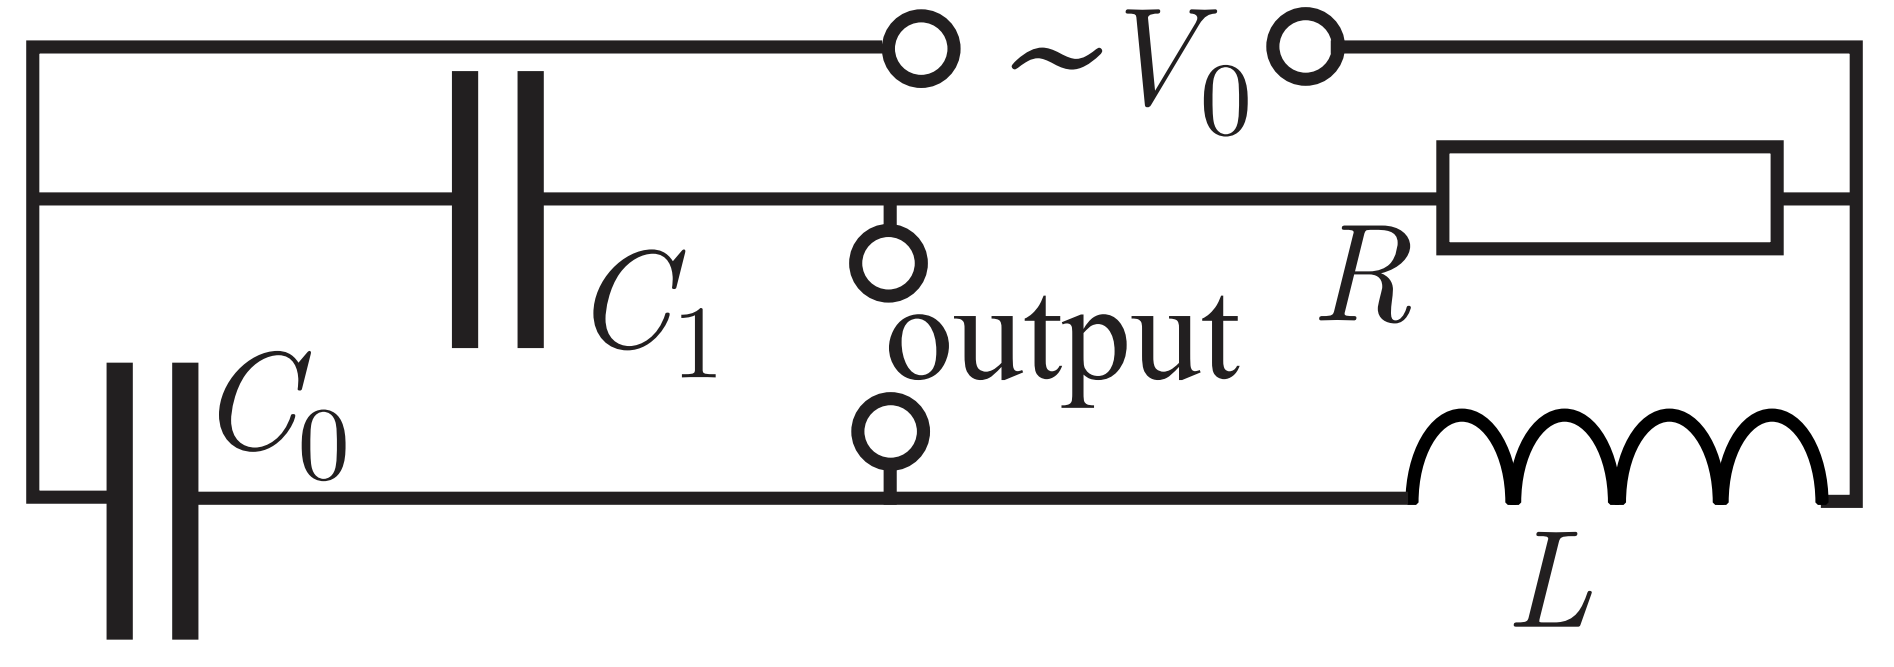
\includegraphics[scale=0.2]{et}
\end{center}
\begin{anum}
    \item For which oscillation frequency $\omega_0$ would the output voltage be infinite?
    \item Now let the oscillation frequency $\omega$ be twice the value found in the previous task, $\omega = 2\omega_0$. The capacitance $C_1$ is chosen such that the phase difference $\varphi$ between the input and output voltages is maximum (parameters $C_0$, $L$ and $R$ are not changed). Find the phase shift $\varphi$ and the output voltage amplitude $V_{\text{out}}$.
\end{anum}
\end{prob}

\begin{sol}
    See solutions \href{https://nbpho.ee/wp-content/uploads/2022/NBPhO_2022_solutions.pdf}{here} (Problem 4). 
\end{sol}

\begin{prob}\label{powah}
    Let the voltage across an alternating voltage source be $\mathcal E(t)=\mathcal E_0\cos\omega t$, and its current $I(t)=I_0\cos(\omega t+\varphi)$. The instantaneous power at any moment is equal to $\mathcal E(t)\cdot I(t)$. Using a trigonometric identity, prove that the average power dissipation in the circuit is $$P=\mathcal E_{\text{rms}}I_{\text{rms}}\cos\varphi$$
\end{prob}

\begin{sol}
    The instantaneous power is \begin{align*}
        \mathcal E(t)\cdot I(t)&=\mathcal E_0I_0\cos(\omega t)\cos(\omega t+\varphi)\\
        &=\mathcal E_0I_0\cos(\omega t)(\cos\omega t\cos\varphi-\sin\omega t\sin\varphi)\\
        &=\mathcal E_0I_0(\cos^2\omega t\cos\varphi-\cos\omega t\sin\omega t\sin\varphi)
    \end{align*}The long-term average of $\cos^2\omega t=1/2$ and the long-term average of $\cos\omega t\sin\omega t=0$. Plugging these in, we conclude $$P=\frac12\mathcal E_0I_0\cos\varphi=\boxed{\mathcal E_{\text{rms}}I_{\text{rms}}\cos\varphi}$$
\end{sol}


\subsection{Challenge Problems}

\begin{prob}[IPhO]
    Initially, a switch $S$ is unshorted in the circuit shown in the figure on the right, a capacitor of capacitance $2C$ carries the electric charge $q_0$, a capacitor of capacitance $C$ is uncharged, and there are no electric currents in both coils of inductance $L$ and $2L$, respectively. The capacitor starts to discharge and at the moment when the current in the coils reaches its maximum value, the switch $S$ is instantly shorted. Find the maximum current $I_{\text{max}}$ through the switch $S$ thereafter.
    \begin{center}
        
\includegraphics[scale=0.2]{ipho2}
    \end{center}
\end{prob}

\begin{sol}
    See solutions \href{https://s3.eu-central-1.amazonaws.com/physprob.com/files/ipho/2014_Kazakhstan_p1Sol.pdf}{here} (Part C).
\end{sol}

\begin{prob}[IPhO]
    Try IPhO 1994, Problem 2 \href{https://s3.eu-central-1.amazonaws.com/physprob.com/files/ipho/1994_China_p2.pdf}{here}.
\end{prob}

\begin{sol}
    See solutions \href{https://s3.eu-central-1.amazonaws.com/physprob.com/files/ipho/1994_China_p2Sol.pdf}{here}.
\end{sol}

\subsection{USAPhO Practice}

\begin{prob}[USAPhO 2018 A2]
    See problem statement and answer sheets \href{https://drive.google.com/file/d/1Ppyd31iieYWaprdalgzkgx8ewSoMahxF/view?usp=sharing}{here} (printable).
\end{prob}

\begin{sol}
    See solutions \href{https://aapt.org/physicsteam/2019/upload/USAPhO-2018-Solutions.pdf}{here}.
\end{sol}

\begin{prob}
    An oscilloscope is a machine that can generate different types of oscillating voltage distributions. You'll use these a lot at camp. 
    \begin{center}  
        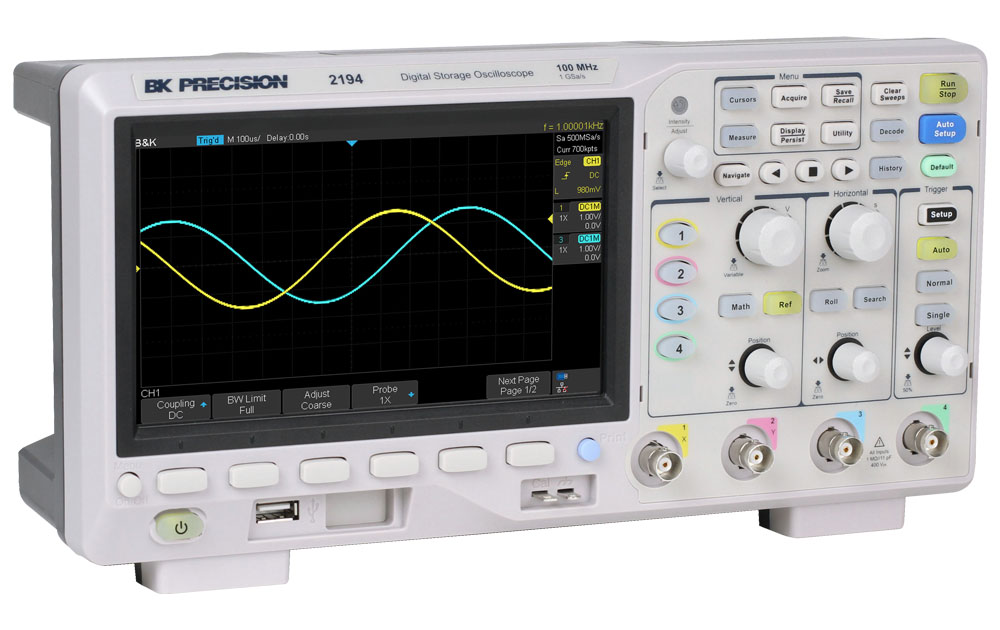
\includegraphics[scale=0.15]{oscilo}
    \end{center}
    We first analyze what happens when the oscilloscope outputs a sinusoidal wave as shown:
    \begin{center}
        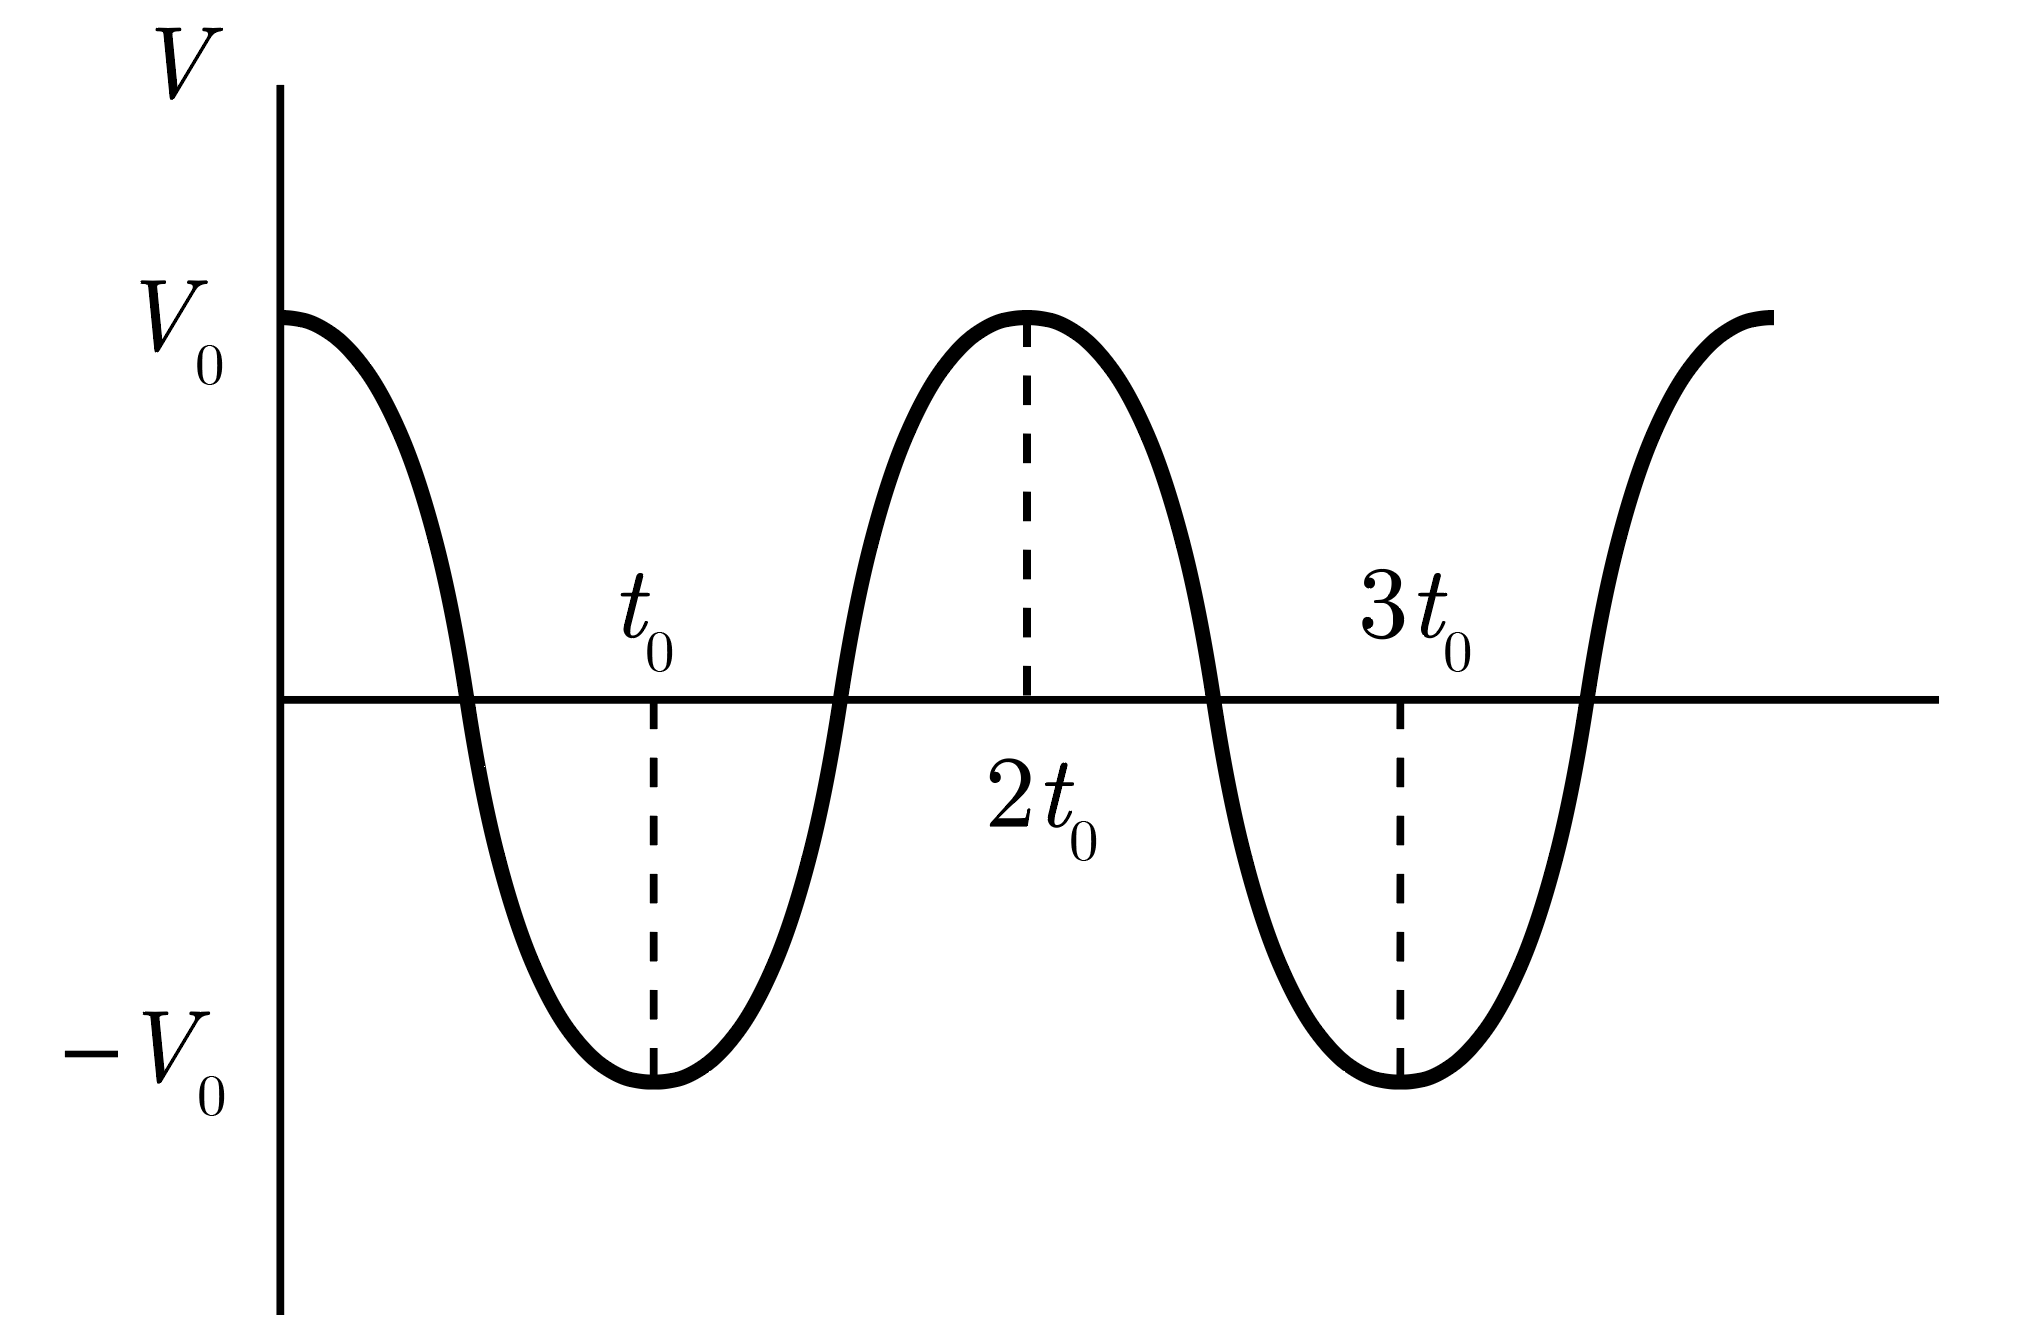
\includegraphics[scale=0.2]{sin}
    \end{center}
    \begin{anum}
        \item Find the RMS voltage of the sinusoidal wave in terms of $V_0$.
        \item The oscilloscope is connected to a series $RC$ circuit. Find the current $I(0)$ at $t=0$. Assume that the sinusoidal curve in the voltage graph above extends infinitely to the left of the graph. 
        \item Over a very long period of time, find the average power supplied by the oscilloscope to the circuit. 
    \end{anum}
    Now we analyze what happens when the oscilloscope outputs a square wave as shown:
    \begin{center}
        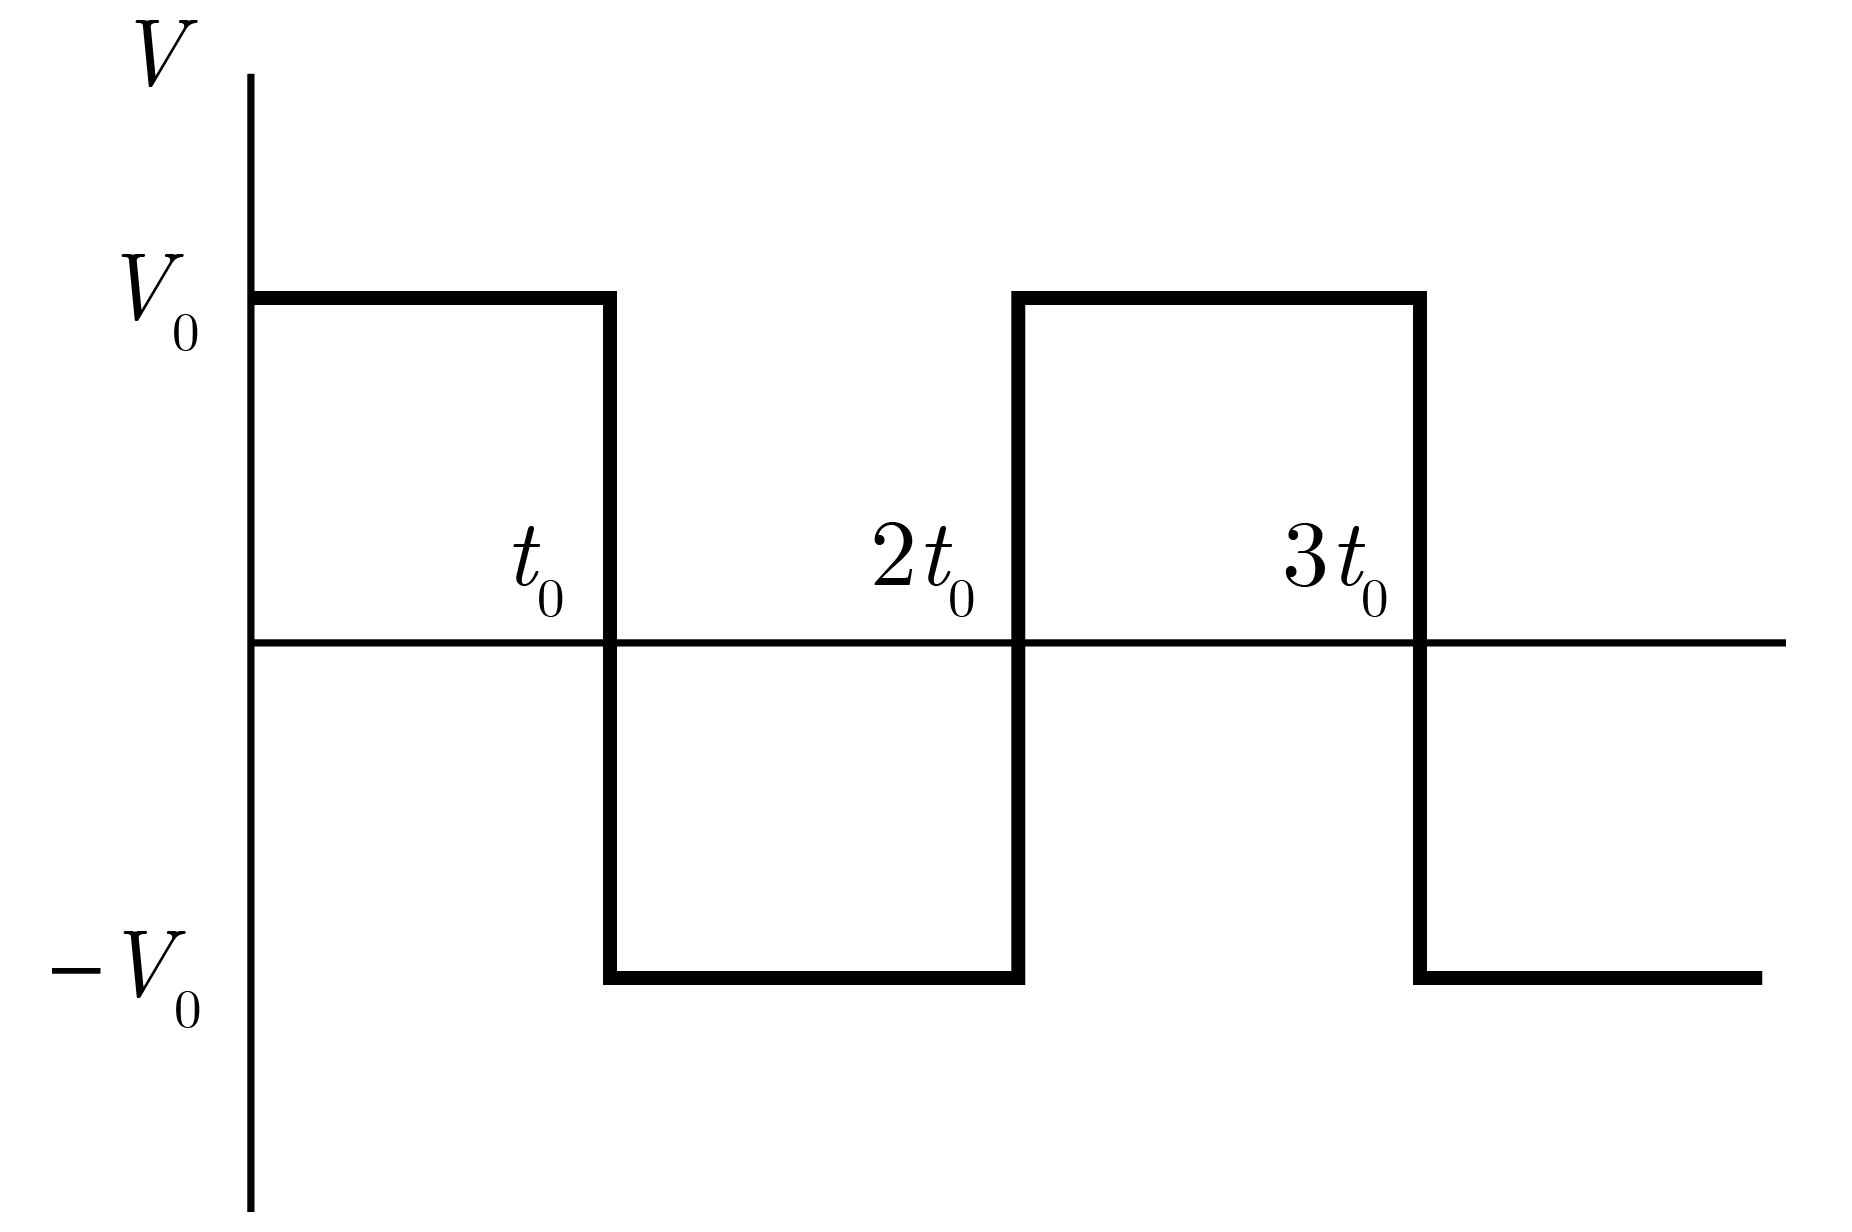
\includegraphics[scale=0.22]{sq}
    \end{center}
    \begin{anum}\addtocounter{enumi}{3}
        \item Find the RMS voltage of the square wave in terms of $V_0$.
        \item The oscilloscope is connected to a series $RC$ circuit, where $RC=t_0$. Assume that at $t=0$, the capacitor carries no charge. Find the current in the circuit immediately after times $t=0$, $t=t_0$, $t=2t_0$, and $t=3t_0$. 
        \item Over a very long period of time, find the average power supplied by the oscilloscope to the circuit. 
    \end{anum}
\end{prob}

\begin{sol}
    \begin{anum}
        \item By the definition of RMS, $$V_{\text{rms}}=\sqrt{\overline{V_0^2\cos^2\omega t}}=\sqrt{\frac{V_0^2}{2}}=\boxed{\frac{V_0}{\sqrt{2}}}$$
        \item Using the phasor method, our diagram is as such: \begin{center}
            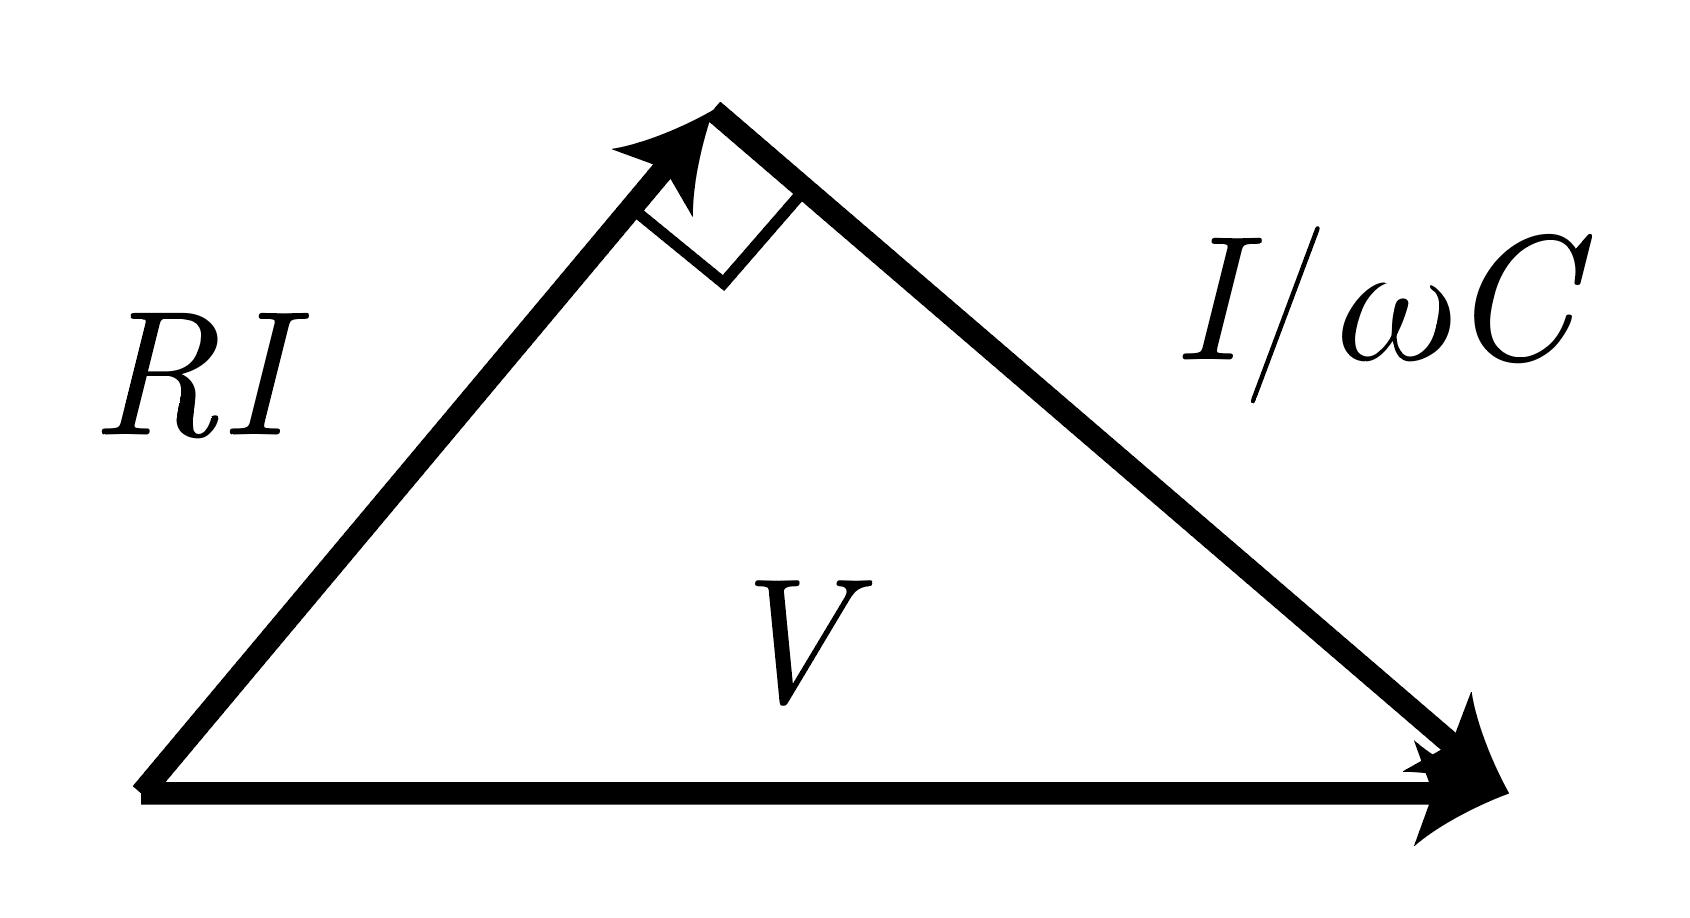
\includegraphics[scale=0.2]{triangle}
        \end{center}
        From the right triangle, the amplitude of $I$ is $I_0=\mathcal E_0/\sqrt{R^2+(1/\omega C)^2}$ and the phase angle is $\varphi=\tan^{-1}(1/\omega RC).$ At $t=0$ the voltage $V$ is set along the real axis as shown, so we simply have $$I(0)=I_0\cos\varphi=\boxed{\frac{\mathcal E_0R}{R^2+1/\omega^2C^2}}$$
        \item From our definition of power, $$P=\frac{\mathcal E_0I_0}{2}\cos\varphi=\boxed{\frac{\mathcal E_0^2R}{2(R^2+1/\omega^2C^2)}}$$
        \item The RMS voltage is simply $V_{\text{rms}}=\boxed{V_0}$. 
        \item At time $t=0$, the current is $I_0=V_0/R$ since there is no voltage on the capacitor. Let $r=1/e$. Since the time constant of the circuit is exactly $t_0$, the current will decay to $rI_0$ at $t=t_0$ right before the switch. At this point the capacitor carries voltage $V_0(1-r)$. When the switch happens, the (magnitude of) voltage on the resistor thus jumps to $V_0(2-r)$. The current then decays again exponentially and becomes $I_0r(2-r)$ before the next switch. After the switch, the current becomes $I_0(2-r(2-r)).$ This pattern continues. To summarize, the results are in the following table (remember $I_0=V_0/R$ and $r=1/e$): \begin{center}
\begin{tabular}{|c|c|}
\hline
$t$ & $I$ \\
\hline 
0 & $I_0$\\
$t_0$ & $I_0(2-r)$\\
$2t_0$ & $I_0(2-r(2-r))$\\
$3t_0$ & $I_0(2-r(2-r(2-r)))$\\
\hline
\end{tabular}
\end{center}
    \item It's clear to see that eventually the magnitude of current (its value measured immediately after each switch) stabilizes. Let this asymptotic value be $xI_0$. Then, it holds that $$2-rx=x\Rightarrow x=\frac{2}{1+r}$$ Now, the average power is the average power dissipated in the resistor. The total energy lost between two switches in the long-term equilibrium is found via $$E=\int_0^{RC}(xI_0e^{-t/RC})^2R\, dt=\left(\frac{2}{1+r}\right)^2I_0^2R\int_0^{RC}e^{-2t/RC}\, dt=\frac{2(1-r)}{1+r}I_0^2R^2C$$ and dividing through by $t_0=RC$, the average power is thus $$P=\frac{2(1-r)}{1+r}\frac{V_0^2}{R}=\boxed{\frac{2(e-1)}{e+1}\frac{V_0^2}{R}}$$
    \end{anum}

\end{sol}

\end{document}